\subsection{DOF \& DOM \& DOF EE}
    \begin{description}
        \item[DOF:] Indep. of Robot Configuration (2D: 3, 3D: 6)
        \item[DOM:] \# Joints
        \item[DOF EE:] Indep. Instant. Motions of End-Effector
    \end{description}
    \subsubsubsection{Grübler's Formula}
        \vspace{0.5em}
        $$
            DOF = C (N-g) + \sum_{i=1}^g f_i
        $$
        \begin{minipage}{0.55\linewidth}
            \begin{description}
                \item[$C$]\,: 3(2D), 6(3D)
                \item[$N$]: \# links w/out baselinks
            \end{description}
        \end{minipage}
        \begin{minipage}{0.44\linewidth}
            \begin{description}
                \item[$f_i$]: \# DOF of $i^{th}$ joint 
                \item[$g$]\,\,: \# joints   
            \end{description}
        \end{minipage}
\subsection{Precision and Accuracy}
    Need more than one measurement to be determined.
    % \vspace{-1em}
    \begin{center}
    	\resizebox{\linewidth}{!}{
    		\includegraphics[
    			page = {3},
    			% trim = {5.8cm, 1.6cm, 5.7cm, 6.75cm}, % with blue frame
    			trim = {6.2cm, 2cm, 6.1cm, 7.15cm}, %left bottom right top
    			clip
    		]{Mechanical_Design/01_2020-09-29_Mechanical-Design.pdf}
    	}
    \end{center}
    \begin{description}
        \item[Precision] "Repeatability" of two+ measurements; $\textrm{std}(M)$ 
        \item[Accuracy] "Closeness" to a standard or known value Accuracy mean; $\textrm{mean}(M) - M_R$
    \end{description}
\subsection{Resolution}
    \textbf{Actuator:} Smallest commendable distance\\
    \textbf{Sensor:} Smallest measurable interval  